% The file is based on the beamer/solutions/conference-talks/
% conference-ornate-20min.en.tex template.

\documentclass{beamer}

\mode<presentation>
{
  \usetheme{Warsaw}
  \setbeamercovered{transparent}
}

\usepackage[english]{babel}
\usepackage[latin1]{inputenc}
\usepackage[T1]{fontenc}

\title
{Current Content Discovery for Business Module Teaching}

\author
{Guanyuming He}

\institute[Imperial College London]
{
  Department of Earth Science and Engineering\\
  Imperial College London
}

\date[IRP 25]
{Independent Research Project, 2025}

% If you have a file called "university-logo-filename.xxx", where xxx
% is a graphic format that can be processed by latex or pdflatex,
% resp., then you can add a logo as follows:

% \pgfdeclareimage[height=0.5cm]{university-logo}{university-logo-filename}
% \logo{\pgfuseimage{university-logo}}


% If you wish to uncover everything in a step-wise fashion, uncomment
% the following command: 

%\beamerdefaultoverlayspecification{<+->}

\begin{document}

\begin{frame}
  \titlepage
\end{frame}

\begin{frame}{Outline}
  \tableofcontents
  % You might wish to add the option [pausesections]
\end{frame}


% Structuring a talk is a difficult task and the following structure
% may not be suitable. Here are some rules that apply for this
% solution: 

% - Exactly two or three sections (other than the summary).
% - At *most* three subsections per section.
% - Talk about 30s to 2min per frame. So there should be between about
%   15 and 30 frames, all told.

% - A conference audience is likely to know very little of what you
%   are going to talk about. So *simplify*!
% - In a 20min talk, getting the main ideas across is hard
%   enough. Leave out details, even if it means being less precise than
%   you think necessary.
% - If you omit details that are vital to the proof/implementation,
%   just say so once. Everybody will be happy with that.

\section{Introduction}

\subsection{Motivation}

\begin{frame}{Business School Case Method}

  \begin{itemize}
  \item
    First institutionalized at Harvard Business School. One of the mainstream
	teaching methods.
  \item
	Engaging for students, but challenging for educators:
	\begin{itemize}
	\item
		Christensen identifies that instructors have to conduct ``extensive
		preparation'' for it.
	\item
		McFarlane emphasises the importance of updated cases, as otherwise
		students could be disengaged or discouraged.
	\end{itemize}
  \end{itemize}
\end{frame}

\begin{frame}{Past advancements in information retrieval}
  \begin{itemize}
	\item No significant improvement until the 19th century.
	\item (Wired) Morse et al.'s telegraph (1840) and Bell's telephone (1876).
	\item (Wireless) Marconi's experiments ($\sim 1900$), first radio voice
		broadcast (1906) 
	\item (Theory) Frequency modulation ($\sim 1930$).  Shannon's bits and
		entropy (1948).   
	\item (Modern) Digital computers, database systems, the Internet.
	\item (Contemporary) Web search engines. Data Science. LLMs.
\end{itemize}
\end{frame}

\subsection{Research aims}
\begin{frame}{But today... So the aims...}
\begin{itemize}
	\item Each of the methods has unique major weaknesses. How well can an
		integration framework be made to compensate each other?
	\begin{itemize}
		\item LLMs struggle at factual accuracy and logical correctness.
		\item Search engines lack semantic or NLP capabilities.
	\end{itemize}
	\item For a module, the main topic is stable. But tools are still manual.
		Aim to improve automation so that only occasional configuration is
		needed.
\end{itemize}
\end{frame}

\section{Methodology}
\subsection{Design philosophy \& Architecture}
\begin{frame}{Design philosophy \& Architecture}
	\begin{center}
		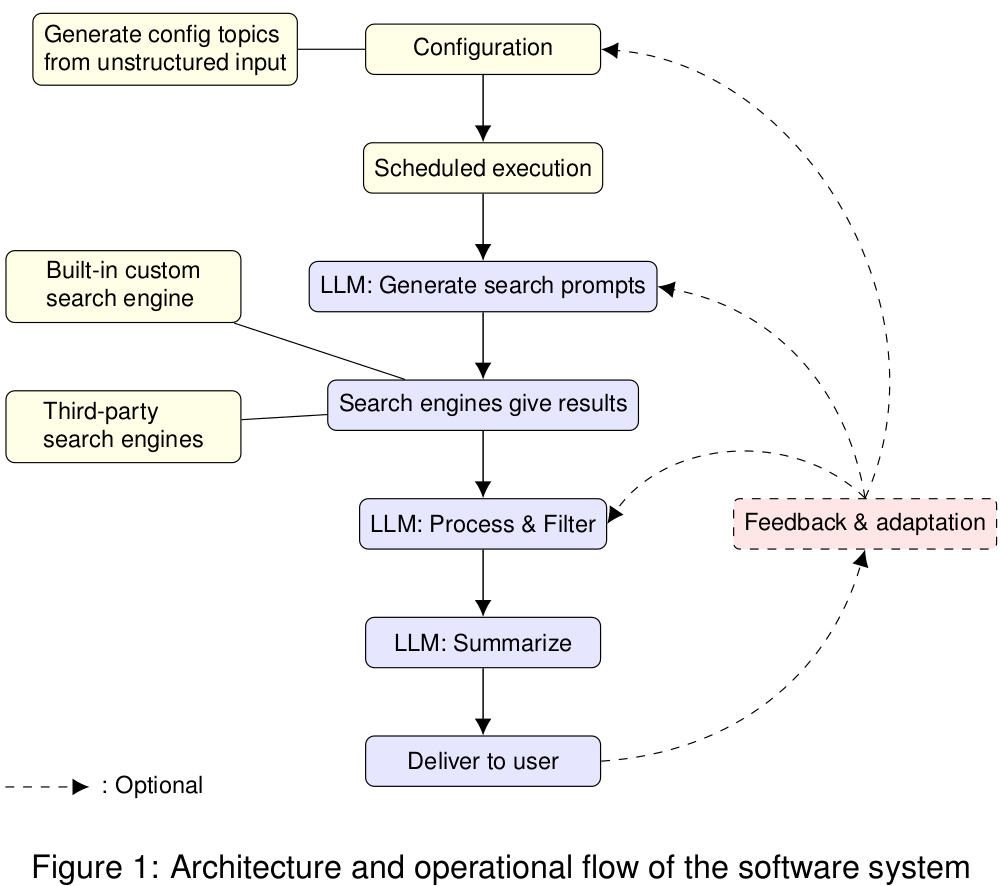
\includegraphics[height=.6\textheight]{./architecture.png}
	\end{center}
	\begin{itemize}
		\item Three software engineering pinciples.
		\item Modular design from the UNIX philosophy; a main pipeline and
			surrounding support programs (scheduling, search engine, GUI).
	\end{itemize}

\end{frame}

\subsection{Technical plans}
\begin{frame}{Technical plans}
	\begin{itemize}
		\item Use C++ (good statically typed) and a number of libraries to
			implement the custom search engine and supporting programs.
		\item Use Python (good scripting for invocation) to implement the rest
			programs.
		\item Use Ollama to invoke LLMs. 
	\end{itemize}
\end{frame}

\section{My results/contribution}
\subsection{Main results}
\begin{frame}{GUI Interface}
	\centering
	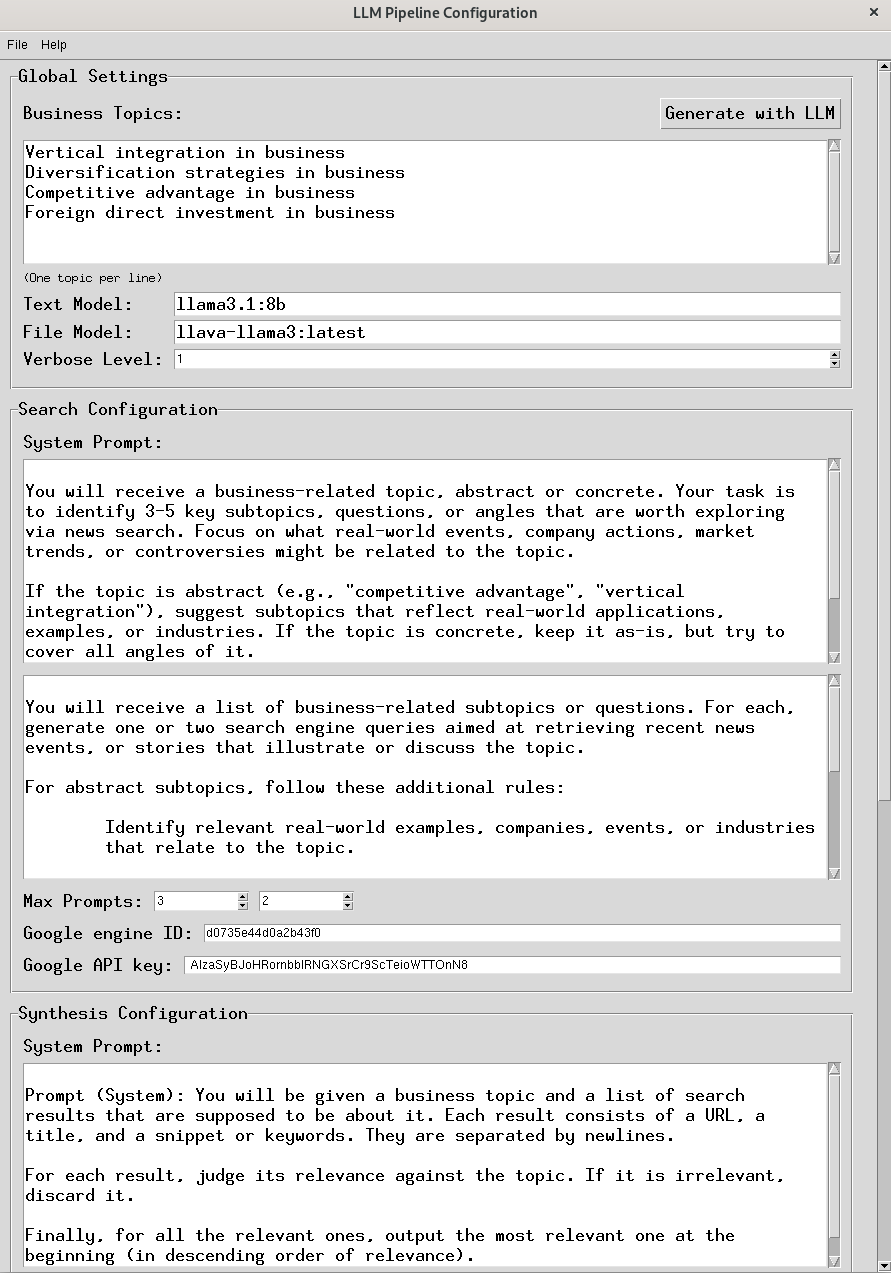
\includegraphics[height=.88\textheight]{../../deliverables/thesis/res/gui.png}
\end{frame}

\begin{frame}{Search Engine}
\begin{itemize}
	\item Custom search engine for explicit and deterministic control.
	\begin{itemize}
	\item Index only reputable Business sites (from online ranking and
		supervisor recommendation)
	\item Can be updated via \texttt{bin/updater} that reads from RSS feeds.
	\end{itemize}
	\item 3rd-party: Google's programmable search engine. Improves coverage.
\end{itemize}
	\vspace{-.6cm}
	\begin{center}
	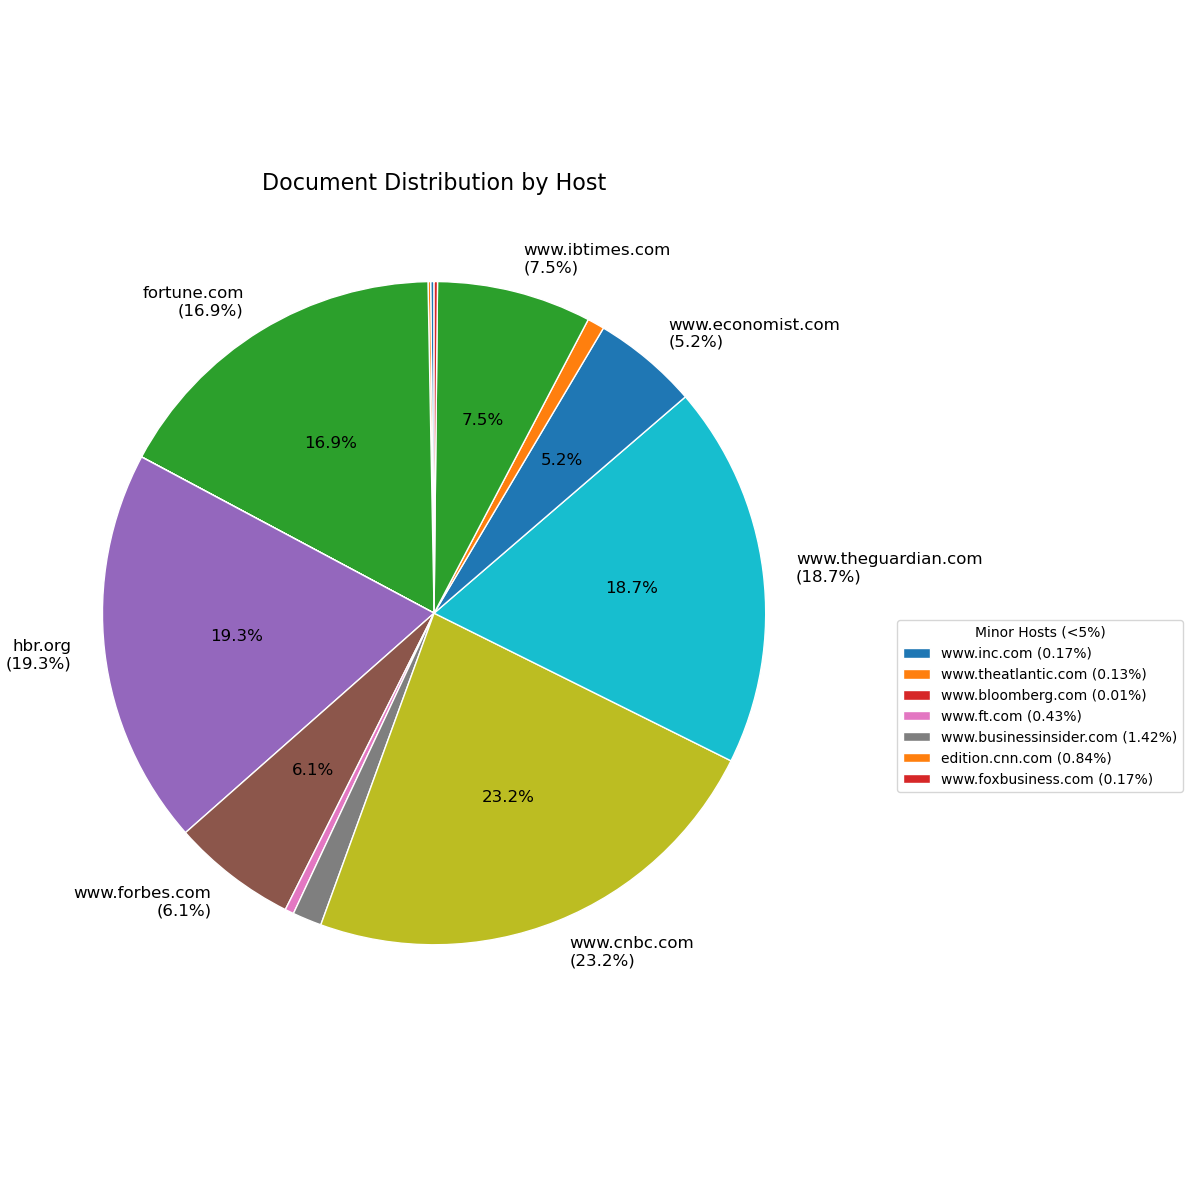
\includegraphics[width=.5\textwidth]{../../deliverables/thesis/res/doc_host_dist.png}
	\end{center}
\end{frame}

\begin{frame}{LLM invocation}
	\begin{itemize}
	\item Multi-stage invocation: 
		\begin{enumerate}
		\item For each business topic, generate subtopics.
		\item For each subtopic, generate search prompts.
		\item For each search result, judge its relevance (return a number)
		\item For the filtered and reranked results, give a summary.
		\end{enumerate}
	\end{itemize}
	\begin{center}
	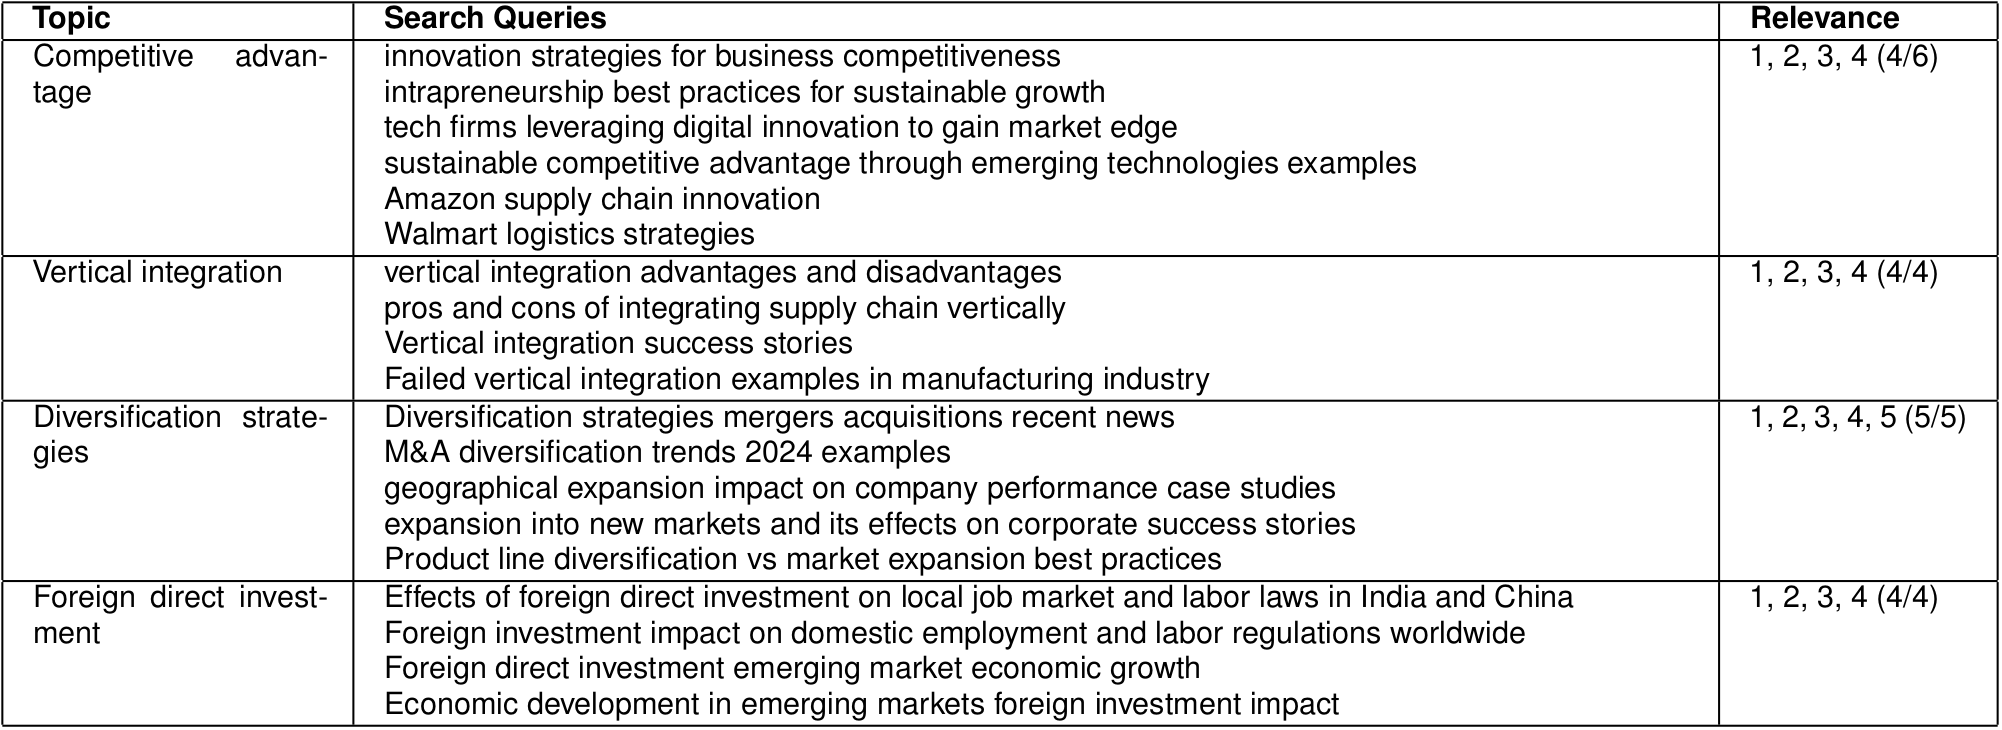
\includegraphics[height=.4\textheight]{../../deliverables/thesis/res/table_search_queries.png}
	\end{center}
\end{frame}

\subsection{Contemporary related work}
\begin{frame}{Works that improve LLMs/Search engines}
	\begin{itemize}
	\item Improve LLMs
	\begin{itemize}
		\item RAG: use pretrained retriever to address hallucination.
		\item Many others use external knowledge to augment LLMs as well. Most
			are to improve question answering.
		\item Perhaps most similar to mine among them: WebGPT, whose retriever
			is not a model, but a web browser that the LLM can use.
	\end{itemize}
	\item Improve search engines
	\begin{itemize}
		\item Some use LLMs to rewrite and improve search queries.
		\item Some assist ranking of search results.
		\item A few use LLMs in the indexing stage for NLP tasks (e.g.\ term
			extraction, meaning filtering).
	\end{itemize}
	\end{itemize}
\end{frame}

\begin{frame}{Overall contribution over similar academic works}
	\begin{itemize}
		\item Designed a novel pipeline that combined search engines and LLMs.
		\item Aimed to address weaknesses of \emph{both} seach engines and
			LLMs. (Similar works almost always aim to address one of them's.)
		\item Developed an \emph{automatic} system that only requires
			occasional user configuration.
	\end{itemize}
\end{frame}

\subsection{Comparsion with mainstream commercial tools}
\begin{frame}{Comparison with ChatGPT and Google}
\begin{itemize}
	\item Versus ChatGPT, my system drastically reduced search
		results of non-reputable sites and kept the results recent. However, my
		system produced a few irrelavant search queries and could not compete
		with ChatGPT in summary quality. 
	\item Against Google, my system retrieved more reputable and current
		information, but lacked in breadth. When Google's AI overview was
		triggered, its summary quality also appeared to be superior.
\end{itemize}
\begin{center}
	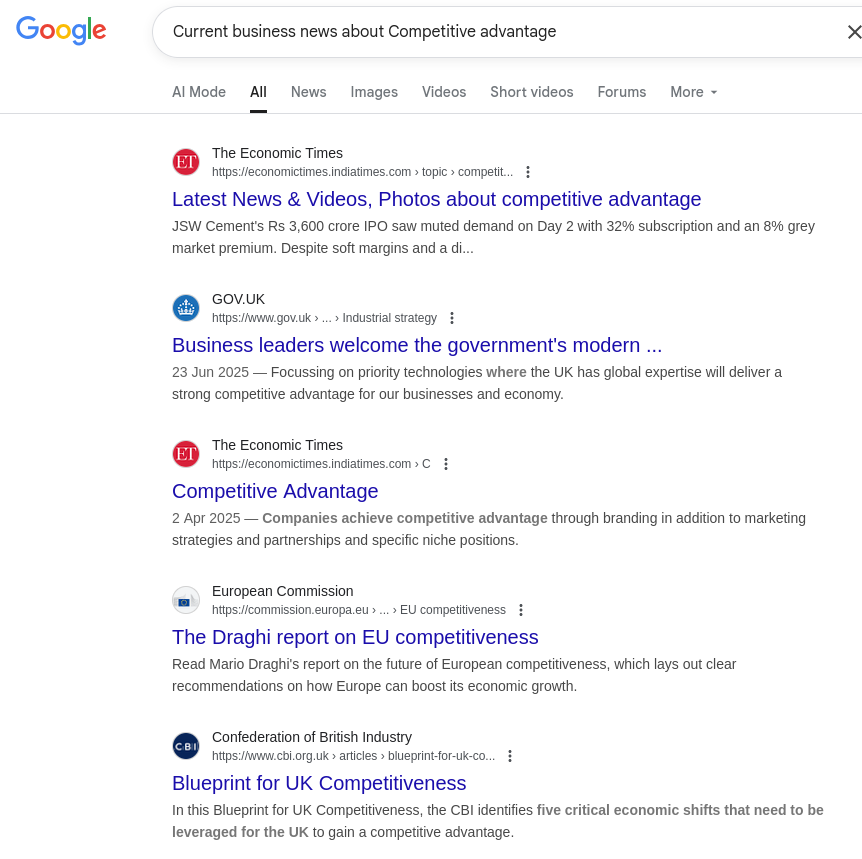
\includegraphics[height=.4\textheight]{../../deliverables/thesis/res/google_res1.png}
	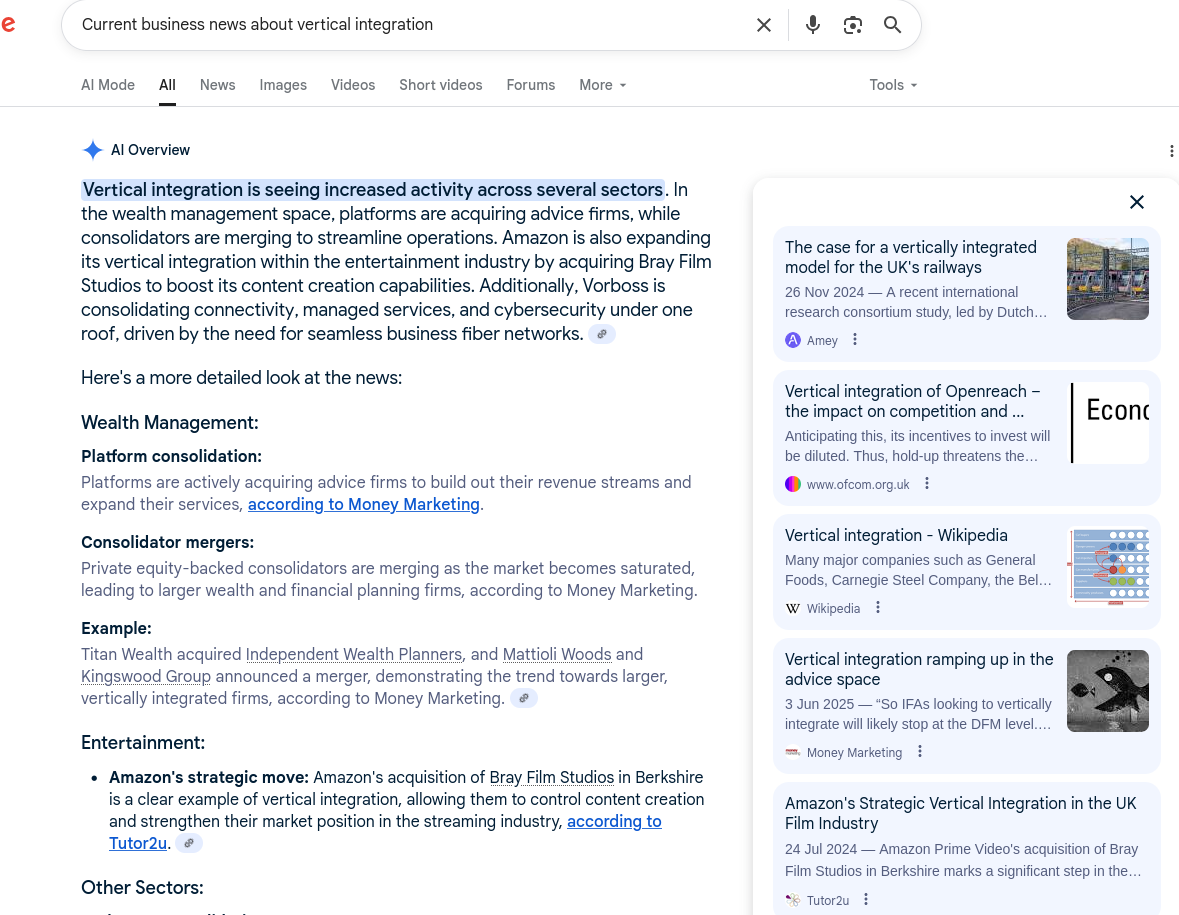
\includegraphics[height=.4\textheight]{../../deliverables/thesis/res/google_res2.png}
\end{center}
\end{frame}

\section*{Challenges \& Future Plans}
\begin{frame}{Challenges \& Future Plans}
  \begin{itemize}
  \item
	  It fails to match the summarization power of commerical AI, probably
	  because it uses local LLMs running on PC.
  \item
	  It is specially tailored to help with business school case method, and a
	  number of places are hard coded for that.
  \item 
	  The custom search engine requires a huge first time setup (indexing).
	  Restrained by PC disk space, its database breadth is also limited.
  \item 
	  My project also does not improve search engines or LLMs theoretically on
	  how they work.
  \item
	  Although judging the summary of business topics is subjective, a dataset
	  and benchmark framework could have been used, but invocation is limited.
  \end{itemize}
\end{frame}

\begin{frame}
	\begin{center}
	{\large THANK YOU!}
	\end{center}

	Further reading:
	\begin{itemize}
		\item Hinrich Sch\"utze, Christopher D Manning, and Prabhakar Raghavan.
			\emph{Introduction to information retrieval}, volume 39.
			Cambridge University Press Cambridge, 2008.
		\item Haoyi Xiong, Jiang Bian, Yuchen Li, Xuhong Li, Mengnan Du,
			Shuaiqiang Wang, Dawei Yin, and Sumi Helal. When search engine
			services meet large language models: Visions and challenges.
			\emph{IEEE Transactions on Services Computing}, 17(6):4558--4577,
			2024.
	\end{itemize}
\end{frame}

\end{document}


